\section{Desenvolvimento}

\subsection{Projeto}
%TODO explicar a finalidade deste projeto
Com a finalidade de oferecer uma referência de desenvolvimento de aplicações
Bluetooth no contexto da Internet das Coisas, foi feito um projeto baseado em
microcontroladores que implementa (\ldots) %TODO

O projeto desenvolvido foi o de uma estação de monitoramento de variáveis
ambientais, que tem como funcionalidade principal a realização de leituras
periódicas de sensores com a transmissão sem fio das variáveis medidas
utilizando o bluetooth low energy. Estes dados, quando recebidos por um scanner
bluetooth, são enviados para a internet.

Para tal, dividiu-se as tarefas em três sistemas diferentes, como mostra a
figura \ref{fig:project_overview}:
a estação de medidas, responsável pela coleta e transmissão das medididas através do
bluetooth, o gateway BLE-Internet, responsável por captar os dados no ar e
enviá-los para a internet, e a infraestrutura online, que recebe a informação e
a armazena on-line.

\begin{center}
	\centering 
	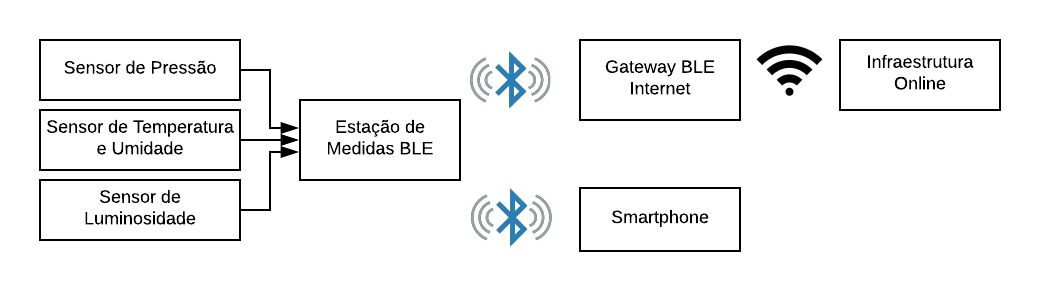
\includegraphics[width=0.5\linewidth]{project_overview.jpg}
	\captionof{figure}{Esquemático dos sistemas presentes no projeto}
	\label{fig:project_overview}
\end{center} 

%TODO justificar as variáveis medidas e os critérios de seleção dos sensores,
% incluindo a disponibilidade de breakout boards

Os sensores escolhidos para o projeto são:
\begin{itemize}
  \item BMP180: Sensor de pressão
  \item TSL2561: Sensor de luminosidade
  \item HTU21D: Sensor de temperatura e umidade
\end{itemize}

Todos os sensores especificados são digitais e possuem características low
power. Além disso, o meio de acesso é o barramento I2C para todos os casos, fato
que auxiliou o desenvolvimento do projeto devido a interface compartilhada entre
todos os dispositivos.

\subparagraph{BMP180} O sensor BMP180, como mostrado no módulo da figura
\ref{fig:bmp180breakout} é um sensor de pressão desenvolvido, produzido e vendido pela Bosch. É capaz de
operar com tensões de 1.8V a 3.6V,consumindo uma corrente de 0.1$\mu A$ a 4$\mu
A$ nas temperaturas de $25\,^{\circ}{\rm C}$ e $85\,^{\circ}{\rm C}$ respectivamente. 
Durante a conversão dos valores de pressão, a corrente de pico varia entre 650$\mu A$ a 1000$\mu A$, e durante a operação a $25\,^{\circ}{\rm C}$ com frequência de amostragem de 1Hz, a
corrente consumida fica entre 3$\mu A$ e 32$\mu A$ dependendo da resolução do
configurada. \cite{BMP180Datasheet}

\begin{center}
	\centering 
	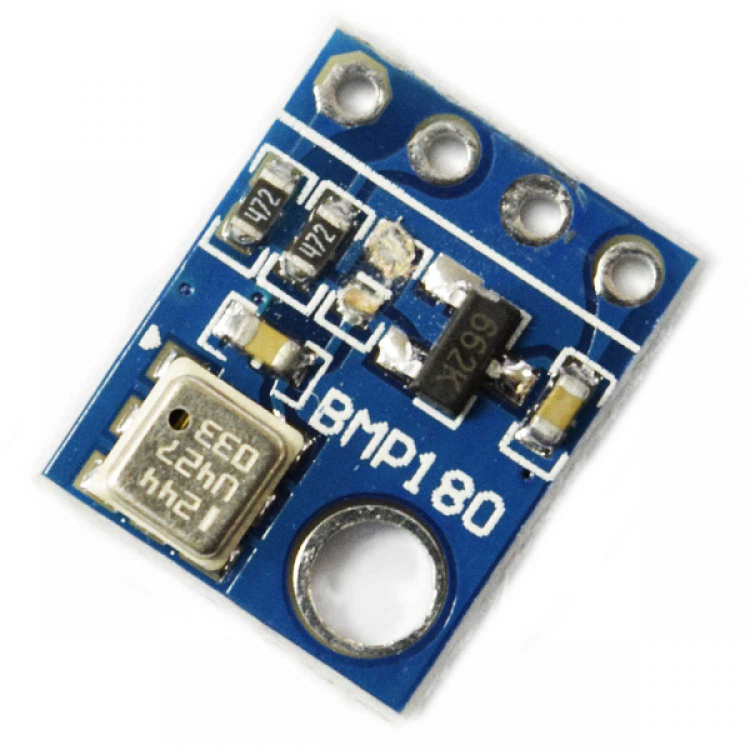
\includegraphics[width=0.5\linewidth]{BMP180.png}
	\captionof{figure}{Módulo de Desenvolvimento para o sensor BMP180}
	\label{fig:bmp180breakout}
\end{center} 


Considerando o tempo máximo de conversão para cada resolução,
estima-se que a frequência de amostragem máxima para este sensor fica entre
222.22Hz(low power mode) e 13Hz(Advanced res. mode). O range de medidas do
sensor é de 30kPa a 110kPa. \cite{BMP180Datasheet}


\subparagraph{TSL2561} O sensor TSL2561,como mostrado na figura
\ref{fig:tsl2561breakout}, é um sensor de luminosidade produzido pela empresa
ams AG que combina um fotodiodo que responde numa larga faixa espectral
(visível e infravermelho) e um fotodiodo que responde somente a faixa
infravermelha do espectro. O sensor possui comunicação I2C que permite a
configuração, leitura e envio de comandos.

\begin{center}
	\centering 
	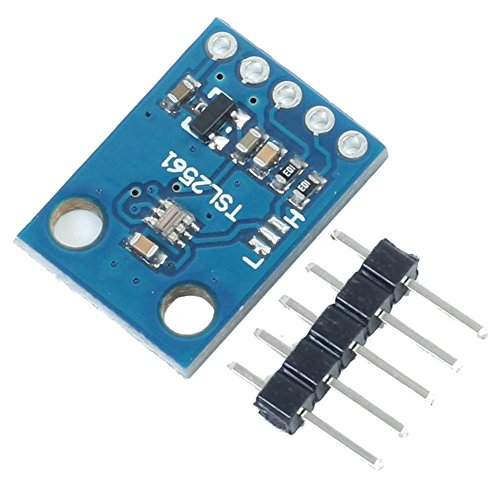
\includegraphics[width=0.4\linewidth]{TSL2561.jpg}
	\captionof{figure}{Módulo de Desenvolvimento para o sensor TSL2561}
	\label{fig:tsl2561breakout}
\end{center} 

Os valores lidos pelo sensor são convertidos para
iluminância em Lux através de uma fórmula empírica que busca se aproximar da
resposta do olho humano. A característica de possuir dois fotodiodos permite
com que o sensor trabalhe em regiões em que há uma incidência alta de luz
infravermelha, pois com um fotodiodo dedicado ao infravermelho é possível medir
e descontar a influência da luz infravermelha na medida de luminosidade.
\cite{TSL2561Datasheet}

A tensão de alimentação é de até 3.8V. Durante os períodos de conversão de
luminosidade, o consumo de corrente varia entre 0.24mA e 0.6mA. Já no modo
power down, o consumo de corrente varia entre 3.2$\mu A$ e 15$\mu A$. Possui
uma resolução de 16 bits na saída do ADC que realiza as conversões nos
fotodiodos. \cite{TSL2561Datasheet}

% \begin{listing}
% For 0 < CH1/CH0 ≤ 0.50
% Lux = 0.0304 × CH0 - 0.062 × CH0 × ((CH1/CH0)1.4)
% For 0.50 < CH1/CH0 ≤ 0.61
% Lux = 0.0224 × CH0 - 0.031 × CH1
% For 0.61 < CH1/CH0 ≤ 0.80
% Lux = 0.0128 × CH0 - 0.0153 × CH1
% For 0.80 < CH1/CH0 ≤ 1.30
% Lux = 0.00146 × CH0 - 0.00112 × CH1
% For CH1/CH0 > 1.30
% Lux = 0
% \end{listing}

\subparagraph{HTU21D} O sensor HTU21D, como mostra a figura \ref{fig:htu21breakout} é um
sensor de temperatura e umidade relativa do ar desenvolvido e produzido pela
Measurement Specialities. Este sensor é low power, sendo capz e operar entre
tensões de 1.5V e 3.6V com um consumo de corrente variando entre 0.02$\mu A$ e
0.14$\mu A$ em standby, e consumindo uma corrente que varia entre 300$\mu A$ a
500$\mu A$ durante a conversão de temperatura e umidade. \cite{HTU21DDatasheet}

\begin{center}
	\centering 
	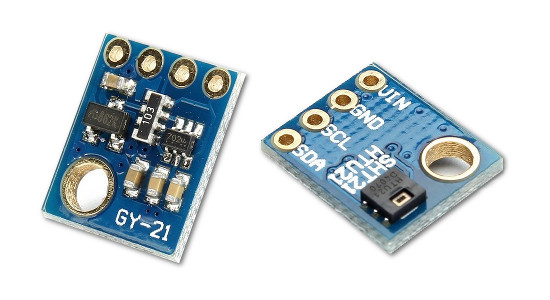
\includegraphics[width=0.4\linewidth]{HTU21.jpg}
	\captionof{figure}{Módulo de Desenvolvimento para o sensor HTU21}
	\label{fig:htu21breakout}
\end{center} 

Possui uma  resolução configurável de 8 bits a 12 bits para a medida de umidade
relativa do ar, que corresponde a 0.7\%RH e 0.04\%RH respectivamente com uma
acurácia de 2\%RH, com duração de conversão é de 3ms (8 bits) a 16ms (12 bits).
O sensor de umidade possui um tempo de resposta de 5 a 10 segundos para uma
excitação em degrau de 33\%RH para 75\%RH. \cite{HTU21DDatasheet}

Já para a medida de temperatura, a resolução é configurável entre 11 bits e 14
bits, representando $0.08\,^{\circ}{\rm C}$ e $0.01\,^{\circ}{\rm C}$
respectivamente, com uma acurácia de $0.3\,^{\circ}{\rm C}$ e com duração da
conversão variando de 7ms (11 bits) a 50ms (14 bits). Possui um tempo de
resposta de 10 segundos para uma excitação em degrau de $15\,^{\circ}{\rm C}$ a
$45\,^{\circ}{\rm C}$.\cite{HTU21DDatasheet}

\subsubsection{Estação de Medidas Bluetooth Low Energy}

A estação de medidas foi projetada para atender os requisitos propostos,
visando o mínimo consumo energético para possibilitar a alimentação através de
baterias sem a necessidade de manutenções frequentes.
 
Como diferencial a estação permite a configuração de sua operação através de
serviços GATT do BLE, sendo possível alterar tanto as configurações de rádio
(potêcia e intervalo de transmissão) quanto os parâmetros de configuração dos
sensores (range, escala, intervalo entre medidas).

O hardware selecionado para a estação de medidas é o SoC nRF51822, produzido
pela Nordic Semiconductor. Este SoC conta com um processador ARM Cortex M0 de 32
bits e com um transceiver de 2.4GHz multiprotocolo, sendo capaz de operar com
os protocolos Bluetooth e ANT.\cite{nRF51ProdSpec}

A plataforma escolhida leva em consideração as especificações energéticas do
SoC, a possibilidade de depuração do código desenvolvido, a versatilidade de
operar tanto a aplicação quanto o bluetooth dentro do mesmo chip e a
disponibilidade do componente para o uso.

\subsubsubsection{Estratégia para otimização de consumo energético}
Com a finalidade de otimizar o consumo energético foi adotada a estratégia de
manter o microcontrolador em modo deep sleep sempre que possível, sendo o mesmo
acordado somente através de interrupções para a realização das tarefas de rádio
e de leitura de sensores. Durante os períodos em sleep todos os sensores devem
estar num estado de baixo consumo de energia.\cite{MicrochipLPDesign}

Ainda na otimização do consumo, a estratégia adotada para a transmissão dos
dados dos sensores foi concepção do dispositivo operando como um BLE advertiser
pois desta forma se reduz o período no qual há a necessidade do rádio, e
somente durante a configuração o dispositivo opera como um BLE Slave,
permitindo que uma conexão seja estabelecida e que os serviços e
características presentes sejam acessíveis.

\subsubsubsection{Bluetooth Advertiser} 
No modo advertiser, o dispositivo transmite a informação de que este aceita o
estabelecimento de conexões com centrais BLE. Além disso, estão presentes nos
pacotes transmitidos as leituras realizadas pelos sensores.

As informações dos sensores são codificadas como payload do pacote seguindo a
estrutura de dados no código fonte \ref{lst:struct_adv}. Como formato de
payload, optou-se por utilizar o Manufacturer Specific Data, evitando assim
possíveis conflitos com pacotes BLE definidos pela especificação.

\lstinputlisting[firstline=11,lastline=18,label={lst:struct_adv},
caption={Estrutura de dados para do pacote de leituras dos sensores}]
{../Development/ble-sensor-station/src/libs/ble/advertising/ble_adv_frame.h}

Os pacotes MSD são definidos na especificação suplementar, sendo o data type
definido como  

% -> Utilização do msd
% A transmissão dos pacotes de advertising são feitos através do formato de
% Manufacturer Specific Data, desta garante-se a compatibilidade dos pacotes
% transmitidos por este dispositivo com a especificação sem causar erro
% 
% Codificação do pacote de advertising

\subsubsubsection{Bluetooth Slave}
No modo slave, o dispostivo possui um serviço Bluetooth para cada sensor, com
características que permitem a configuração dos sensores.

O UUID de 128 bits,arbitrariamente utilizado como base para
todos os serviços, está descrito no código fonte \ref{lst:base_uuid}.

\lstinputlisting[firstline=11,lastline=15,label={lst:base_uuid},
caption={Constante que define o UUID base dos serviços Bluetooth}]
{../Development/ble-sensor-station/src/libs/ble/services/ble_services_common.h}

Este UUID foi construído convertendo para hexadecimal o código ASCII da mensagem
\dblquote{UFABCIAR2018\_\_GN}, onde os caracteres \dblquote{\_\_} são os bytes
$0x00$ deixados em branco para o preenchimento pelo UUID específico dos serviços
bluetooth.

Foram definidos e nomeados quatro serviços Bluetooth para o dispositivo: o APSS
(Air Pressure Sensor Service), o LSS (Luminosity Sensor Service), o THSS
(Temperature and Humidity Sensor Service) e o RPCS (Radio Parameters
Configuration Service).

\subparagraph{Air Pressure Sensor Service}(APSS) 
\newline
O APSS é o serviço responsável pela configuração do sensor de pressão BMP180.
Este sensor disponibiliza via Bluetooth as informações de pressão atmosférica e
temperatura. Este serviço possui 5 características: Sensing Interval, Sensor
Status, Sensor Resolution, Pressure Data, Temperature Data. Os identificadores
de 2 bytes do serviço e de cada característica estão definidos no Código Fonte
\ref{lst:apss_uuid}. 

\lstinputlisting[firstline=19,lastline=29,label={lst:apss_uuid},
caption={UUID para o serviço APSS e suas características}]
{../Development/ble-sensor-station/src/libs/ble/services/apss/ble_apss.h}

A característica Sensing Interval é uma característica que representa o
intervalo entre as medidas de pressão e temperatura do sensor de BMP180
configurada atualmente. Possui exatamente 4 bytes, o suficiente para armazenar
uma variável do tipo \textbf{uint32\_t}, que representa o intervalo em
milisegundos.

Ao realizar a leitura desta característica, se obtém o intervalo atual entre as
medidas do sensor, e a escrita nesta característica realiza uma nova
configuração. A leitura é permitida sem restrições, já escrita passa pelo
processo de autorização para rejeitar a configuração em caso de valor
inválido. Neste projeto não foi previsto nenhum valor inválido para o intervalo
entre as medidas, porém este recurso possibilita a implementação com menor
retrabalho de software.

A característica Sensor Status indica o estado atual do sensor. Foram previstos
3 estados diferentes para o sensor, como mostra o Código Fonte
\ref{lst:sensor_state_t}. Esta característica possui 1 byte de comprimento, que
pode ser lido a qualquer momento ou escrito com restrições. Os valores aceitos
para a escrita são 0x00 para ligar o sensor e 0x02 para
desligar o sensor.

Os valores definidos são atribuidos pela construção de uma estrutura do tipo
enumeração, sendo o primeiro elemento atribuido com o valor inteiro 0, e
cada novo elemento soma-se 1 unidade ao valor atribuído, conforme
a especificação do enum para a linguagem C.\cite{C99Spec}

\lstinputlisting[firstline=42,lastline=47,label={lst:sensor_state_t},
caption={Enumeração dos possíveis estados para o sensor}]
{../Development/ble-sensor-station/src/libs/sensing/sensor_public_interface.h}

A característica Sensor Resolution determina a resolução e o modo de operação do
sensor. Nesta característica com comprimento de 1 byte, permite-se a leitura sem
restrições e a escrita com validação do valor configurado. Os valores aceitos
para a escrita estão definidos pela enumeração do Código Fonte \ref{lst:bmp180_pwr_mode_t}.
\cite{BMP180Datasheet}

\lstinputlisting[firstline=14,lastline=21,label={lst:bmp180_pwr_mode_t},
caption={Enumeração dos modos de operação configuráveis para o sensor BMP180s}]
{../Development/ble-sensor-station/src/libs/sensing/bmp180_drv/bmp180_drv.h}

As características Pressure Data e Temperature Data são responsáveis pela
transmissão das leituras realizadas pelos sensores. Nelas, armazena-se somente a
leitura mais recente dos sensores sem o acesso ao histórico de leituras. Estas
características permitem apenas a leitura, sem a possibilidade de escrita.
Também é permitido a habilitar o recurso de Notify, que inicia a transmissão dos
dados lidos dos sensores para o dispositivo conectado sem uma solicação de
leitura, operando num sistema de streaming de dados sempre que uma nova leitura
é realizada.

A característica Pressure Data possui 4 bytes de comprimento, transmitindo os
dados num formato \textbf{uint32\_t}, representando a pressão atmosférica em Pa.
Já a Temperature Data, o comprimento é de 2 bytes, transmitindo a temperatura
num formato \textbf{int16\_t}, sendo que cada unidade representa
$0.01\,^{\circ}{\rm C}$ 

\subparagraph{Luminosity Sensor Service}(LSS) 
\newline

\subparagraph{Temperature and Humidity Sensor Service}(THSS) 
\newline

%End of Sensor Station
\subsubsection{Gateway Bluetooth - Internet}

\subsubsubsection{Especificação}

\subsubsubsection{Bluetooth Observer}

\subsubsubsection{Conectividade}

%end of BLE-Internet gateway
\subsubsection{Infraestrutura online}

\subsubsubsection{Servidor para recepção}

\subsubsubsection{Armazenamento e Visualização}
%end of infrastructure
%end of project
\subsection{Implementação}

\subsubsection{Estação de Medidas Bluetooth Low Energy}

% A estação de medidas foi desenvolvida utilizando o SoC NRF51822, produzido pela Nordic
% -> Hardware
% -> Microcontrolador
% -> Sensores		

\subsubsubsection{Ambiente de desenvolvimento}
O ambiente de desenvolvimento foi baseado no Software Development Kit oferecido
pelo fabricante do microcontrolador, o nRF5 SDK 12.3. Este SDK acelera o
desenvolvimento do projeto por diminuir a necessidade de acesso direto aos
registradores do microcontrolador para a operação de hardware, permitindo uma
programação em nível mais elevado.
 
O projeto de firmware foi feito utilizando-se Makefile e o toolchain ARM-GCC,
permitindo assim o desenvolvimento e compilação do projeto de forma
independente de IDE.

A IDE utilizada ao para o desenvolvimento foi o Eclipse IDE versão Oxygen. Além
disso, foram necessárias as ferramentas NRFJPROG, software desenvolvido pelo
fabricante do microcontrolador para realizar tarefas como gravação, leitura,
apagar memória, etc., e a ferramenta Segger J-Link, como interface entre o
computador e o microcontrolador para as operações do NRFJPROG e para a
depuração do firmware.
 
\subsubsubsection{Firmware}

% Estratégia de firmware orientado a eventos
% Linhas gerais sobre firmware para sensores
% Serviços ble
% ADV Encoder/decoder

%End of Sensor Station

\subsubsection{Gateway Bluetooth - Internet}
% 			-> Hardware
% 			-> Ambiente de desenvolvimento
%end of BLE-Internet gateway

\subsubsection{Infraestrutura online}
-> Ambiente de desenvolvimento	
-> Coleta e armazenamento de dados
%end of infrastructure
%end of implementation
